\chapter{Experimental Results} \label{sec:results}
\section{Comparison to algorithms that can solve problems with linear constraints}

In this section we provide experimental comparisons on 22 linearly constrained problems comparing the SHGO, TGO, Lc-DISIMPL \citep{Paul2016}, PSwarm \citep{Vaz2008} and DIRECT-L1 \citep{finkel2003direct} algorithms. Note that the data for the Lc-DISIMPL, PSwarm and DIRECT-L1 algorithms was taken from \citet{Paul2016}. The same error of $pe = 0.01\%$ used by \citet{Paul2016} was also used in this publication. To provide a fair comparison of TGO to SHGO and the other solvers the TGO algorithm was modified to stop sampling when it produced a minimiser that lead to the global minimum of the problem. Table \ref{tab:lc_results} shows the results. Here f.e. is the total number of objective function evaluations required to solve the function and p.f.e. is the total number of penalty function evaluations. \citet{Paul2016} used DIRECT-L1 with the 3 different penalty parameters (p.p.) shown in the table. The PSwarm solver was run 10 times for each test problem. 

The SHGO-Simpl, SHGO-Sobol and TGO (using Henderson's formula for $k_c$) algorithms were able to solve all 22 problems. The lowest average number of function evaluations was achieved by SHGO-Simpl followed by SHGO-Sobol and TGO. It can be observed that Lc-DISIMPL-v achieved a better performance than any other algorithm for the horst-1 to horst-6, hs024, hs035, s232, s250 and bunnag2 problems. As noted in \citet{Paul2016} the initial triangulation of Lc-DISIMPL-v evaluates the function values at the vertices of the simplices and therefore for some of the tested problems the solutions were found after initial triangulation on one of the vertices of the feasible region. It is also possible to initiate SHGO with such an initial triangulation by definition the first few vertices in $\mathcal{X}$ as the intercepts of the linear constraints in a similar way to \citet{Paul2016} and then continuing to add sampling points as normal.

Table \ref{tb:lc} provides additional information for SHGO and TGO including the total number of function evaluations required by the algorithm to solve the problem (f.e.), the number of minimisers generated as starting points by the algorithm (nlmin), the number of unique local minima mapped by the algorithm (nulmin) and the total processing time (runtime) in seconds.

It can be seen that neither of the SHGO algorithms produced more starting points leading to the same local minima as predicted by the theory for adequately sampled function surfaces. On the contrary TGO produced more than one starting point in the same locally convex domain on some test problems which lead to extra function evaluations, producing a poorer overall performance. While SHGO-Simpl had the lowest number of average function evaluations, a higher processing run time is observed compared to the other 2 algorithms. This can be explained by the fact the triangulation code for the sampling has, not yet been optimised, which consumed most of the run time. SHGO-Sobol and TGO use the same sampling generation code and it is observed that SHGO-Sobol has a lower processing run time as expected.


The source code used to produce these results including the scripts that run the test benchmarking suite is publically available at \citet{SHGOpy}. The specifications of the system used to run the test problems can be found in Appendix~\ref{sec:nres}.



\setlength{\tabcolsep}{5.5pt}
\begin{landscape}
% \hspace*{-3cm} 
\begin{table}[htbp]
\caption{Function evaluation comparisons for test problems with linear constraints. }%The results for the Lc-DSIMPL, PSwarm and DIRECT-L1 algorithms were taken from \citet{Paul2016}}
%{\tablinesep=2ex\tabcolsep=10pt
\begin{tabular}{lrrrrrrrrrrrrrr}
\toprule
 & \multicolumn{1}{l}{shgo-}  & \multicolumn{1}{l}{} & \multicolumn{1}{l}{tgo}  & \multicolumn{2}{l}{Lc-DSIMPL-$^c$}   & \multicolumn{1}{l}{PSwarm$^c$} & \multicolumn{1}{l}{} & \multicolumn{1}{l}{} & \multicolumn{1}{l}{}  & \multicolumn{1}{l}{} & \multicolumn{1}{l}{} & \multicolumn{2}{l}{DIRECT-L1$^c$}  &  \\  \cmidrule(lr){7-12}
 & \multicolumn{1}{l}{-simpl}  & \multicolumn{1}{l}{-sobol} & \multicolumn{1}{l}{}  & \multicolumn{1}{l}{-v} & \multicolumn{1}{l}{-c} & \multicolumn{1}{l}{Minimum} & \multicolumn{1}{l}{} & \multicolumn{1}{l}{Average} & \multicolumn{1}{l}{} & \multicolumn{1}{l}{Maximum} & \multicolumn{1}{l}{} & \multicolumn{1}{l}{p.p. = 10} & \multicolumn{1}{l}{p.p. = 10$^2$} & \multicolumn{1}{l}{p.p.=10$^6$} \\  \cmidrule(lr){2-3} \cmidrule(lr){4-4}  \cmidrule(lr){5-6} \cmidrule(lr){7-8} \cmidrule(lr){9-10} \cmidrule(lr){11-12}  \cmidrule(lr){13-15}
Problem & \multicolumn{1}{l}{f.e.} & \multicolumn{1}{l}{f.e.} & \multicolumn{1}{l}{f.e.} & \multicolumn{1}{l}{f.e.} & \multicolumn{1}{l}{f.e.} & \multicolumn{1}{l}{f.e.} & \multicolumn{1}{l}{p.f.e} & \multicolumn{1}{l}{f.e.} & \multicolumn{1}{l}{p.f.e.} & \multicolumn{1}{l}{f.e.} & \multicolumn{1}{l}{p.f.e} & \multicolumn{1}{l}{f.e} & \multicolumn{1}{l}{f.e.} & \multicolumn{1}{l}{f.e.} \\ 
\midrule
horst-1  & 97 & 24 & 34 & 7 & 249 & 167 & 182 & 1329$^{b(3)}$ & 1343$^{b(3)}$ & 4100$^{b(3)}$ & 4101$^{b(3)}$ & 287$^a$ & 3689 & $>$100000 \\[0.05cm]
horst-2  & 10 & 11 & 11 & 5 & 171 & 160 & 176 & 424 & 492 & 768 & 867 & 265$^a$ & 10829 & $>$100000 \\[0.05cm]
horst-3  & 6 & 7 &  6 & 5 & 249 & 42 & 43 & 44 & 45 & 46 & 47 & 5$^a$ & 591 & 617 \\[0.05cm]
horst-4  & 10 & 25 & 24 & 8 & 260 & 90 & 179 & 114 & 194 & 129 & 211 & 58293$^a$ & $>$100000 & $>$100000 \\[0.05cm]
horst-5  & 20 & 15 & 15 & 8 & 259 & 106 & 150 & 134 & 192 & 214 & 302 & 7$^a$ & $>$100000 & $>$100000 \\[0.05cm]
horst-6  & 22 & 59 & 77 & 10 & 284 & 90 & 172 & 110 & 192 & 133 & 227 & 11$^a$ & 739$^a$ & $>$100000 \\[0.05cm]
horst-7  & 10 & 15 & 13 & 10 & 220 & 188 & 201 & 380 & 403 & 919 & 957 & 7$^a$ & 71$^a$ & $>$100000 \\[0.05cm]
hs021  & 24 & 23 & 23 & 189 & 133 & 110 & 110 & 189 & 192 & 392 & 405 & 97 & 97 & 97 \\[0.05cm]
hs024  & 24 & 15 & 36 & 3 & 141 & 101 & 153 & 118 & 172 & 138 & 195 & 19$^a$ & 57$^a$ & $>$100000 \\[0.05cm]
hs035  & 37 & 41 & 35 & 630 & 721 & 266 & 311 & 316 & 369 & 327 & 373 & $>$100000 & $>$100000 & $>$100000 \\[0.05cm]
hs036  & 105 & 20 & 103 & 8 & 314 & 179 & 179 & 396 & 401 & 561 & 574 & 25$^a$ & 49$^a$ & $>$100000 \\[0.05cm]
hs037  & 72 & 63 & 258 & 186 & 9129 & 127 & 131 & 160 & 167 & 201 & 574 & 7$^a$ & 7$^a$ & $>$100000 \\[0.05cm]
hs038  & 225 & 1029 & 389 & 3379 & $>$100000 & 53662 & 54445 & 58576 & 59821 & 65677 & 67660 & 7401 & 5885 & 6511 \\[0.05cm]
hs044  & 199 & 35 & 51 & 20 & 440 & 148$^{b(9)}$ & 218$^{b(9)}$ & 186$^{b(9)}$ & 281$^{b(9)}$ & 201$^{b(9)}$ & 299$^{b(9)}$ & 90283 & $>$100000 & $>$100000 \\[0.05cm]
hs076  & 56 & 37 & 44 & 548 & 4794 & 132 & 198 & 203 & 286 & 275 & 341 & 19135 & $>$100000 & $>$100000 \\[0.05cm]
s224  & 166 & 165 & 165 & 49 & 463 & 105 & 107 & 121 & 122 & 157 & 158 & 7$^a$ & 431 & 457 \\[0.05cm]
s231  & 99 & 99 & 383 & 2137 & 655 & 542 & 1011 & 2366 & 3020 & 4116 & 4800 & 1261 & 1209 & 43341 \\[0.05cm]
s232 & 24 & 15 & 22 & 3 & 141 & 105 & 144 & 119 & 171 & 162 & 236 & 19$^a$ & 57$^a$ & $>$100000 \\[0.05cm]
s250 & 105 & 20  & 103 & 8 & 314 & 296 & 296 & 367 & 375 & 495 & 498 & 25$^a$ & 49$^a$ & $>$100000 \\[0.05cm]
s251 & 72 & 63 & 258 & 186 & 9127 & 83 & 84 & 129 & 137 & 175 & 180 & 7$^a$ & 7$^a$ & $>$100000 \\[0.05cm]
bunnag1  & 34 & 47 & 39 & 630 & 721 & 132 & 142 & 214 & 228 & 411 & 438 & 1529 & 1495 & 1463 \\[0.05cm]
bunnag2  & 46 & 36 & 35 & 16 & 500 & 150 & 153 & 252 & 259 & 410 & 426 & $>$100000 & $>$100000 & $>$100000 \\[0.05cm]
\cmidrule(lr){2-15}
Average  & 66 & 88 & 100 & 366 & $>$5877 & 2590 & 2672 & 3011 & 3130 & 3637 & 3812 & $>$17213 & $>$28421 & $>$75113 \\[0.05cm]
\bottomrule
\end{tabular}
\begin{tabular}{l}
$a$ result is outside the feasible region \\
$b(t)$ $t$ out of 10 times the global solution was not reached \\
$c$ results produced by \citeauthor{Paul2016} (\citeyear{Paul2016})
\end{tabular}
%}
 \label{tab:lc_results}
\end{table}
\thispagestyle{plain}
\end{landscape}


\begin{table}[htbp]
\caption{Total and average performance over all 22 test problems.}
\begin{tabular}{llrrrr}
\toprule
    &                &  f.e. &  nlmin &  nulmin  &   runtime (s) \\
problem & name        &       &        &                  &           \\
\midrule
All & shgo-simpl     &  1463 &     26 &      26  &       0.27294 \\
    & shgo-sobol       &  1864 &     23 &      23 &       0.11225 \\
    & tgo       &  2123 &     29 &      25  &       0.093607 \\
Average & shgo-simplicial      &    65 &      1 &       1  &  0.012852 \\
    & shgo-sobol       &    88 &      1 &       1  &  0.004144 \\
    & tgo      &    100 &      1 &       1  &  0.004542 \\
\bottomrule
\end{tabular}
\label{tb:lc}
\end{table}

\section{Function evaluations and comparison to other open source global optimisation algorithms}
In this section we present numerical experiments comparing the SHGO and TGO algorithms with the SciPy implementations \citep{scipy} of basinhopping (BH) \citep{li1987monte, wales2003energy, wales1997global, wales1999global} and differential evolution (DE) \citep{Storn1997}. These algorithms were chosen both because the open source versions are readily available in the SciPy project and because BH is commonly used in energy surface optimisations \citep{Wales2015} from which the motivation for developing SHGO grew. DE has also been applied in optimising Gibbs energy surfaces for phase equilibria calculations \citep{Zhang2011}. The optimisation problems in Appendix~\ref{sec:nres} were selected from the SciPy global optimisation benchmarking test suite \citep{Adorio2005, Gavana2016, Jamil2013, Mishra2007, Mishra2006, NIST2016}. The test suite contains multi-modal problems with box constraints, they are described in detail in \citet{Gavana2016}. We again used the stopping criteria $pe = 0.01\%$ for SHGO and TGO. For the stochastic algorithms (BH and DE) the starting points provided by the test suite were used. For every test the algorithm was terminated if the global minimum was not found after 10 minutes of processing time and the test was flagged as a fail. For comparisons we used normalised performance profiles \citep{Dolan2002} using function evaluations and processing time as performance criteria. In total 180 test problems were used.

From \Cref{fig:pprofile} it can be observed that for this problem set SHGO-Sobol was the best performing algorithm, followed closely by TGO and SHGO-Simpl. \Cref{fig:pprofilezoom} provides a clearer comparison between these three algorithms. While the performance of all 3 algorithms are comparable, SHGO-Sobol tends to outperform TGO, solving more problems for a given number of function evaluations. This is expected since, for the same sampling point sequence, TGO produced more than one starting point in the same locally convex domain on some test problems which leads to extra function evaluations. In total TGO produced 403 minima of which only 393 minima were unique while all of the 225 minima produced by SHGO-Sobol were unique. SHGO-Simpl produced 238 of which all 238 were unique. It is apparent that SHGO-Simpl performed worse compared to the other sampling methods despite a better performance on the test problem set with linear constraints. There are two reasons for this result. First of all, the uniformity properties of the Sobol sequence hold only for hypercubes. Therefore, it is lost for geometries defined by the search spaces inside linear constraints. Secondly the current code for the triangulation of the simplex cannot add only one sampling point per iteration, but must split all the simplices until the symmetry of the entire complex is restored. This leads to a much higher number of function evaluations during the sampling step of the algorithm.

\Cref{tab:results} in Appendix~\ref{sec:nres} shows the raw numerical results. Note that, unlike the data in performance profiles, failed test runs did not get set to the worst case performance criteria by any solver (in order to preserve the raw data). Therefore the total and average function evaluations and processing times are misleading. The Table is mostly useful for comparisons on a particular test problem as well as comparing the total number of minima and unique minima found.



%From the results it should first be noted that not all of the 1035 starting minimisers produced by SHGO algorithm lead to unique local minima (of which  944 is found across all the problems), this is both due to the fact that the 100 initial sampling points were inadequate for many of the problems and that the local minimisation was not supplied with the set of bounds provided by the boundary of the $k-$chain around $\textrm{st}\left( v_i \right)$,  $\partial \left( C(\mathcal{H}^k) \right), k = n + 1$, and could therefore jump outside the locally convex domain in the local minimisation step. Furthermore some of the problems in the  test suite are not smooth functions. Of the 895 starting minimisers produced by TGO algorithm only 749 unique minima were found. Overall SHGO used less functions evaluations per number of unique minima discovered (123.99) compared to TGO (136.82).  However, TGO used less function evaluations overall since SHGO used more local minimisation evaluations to find more unique local minima.


\begin{figure} %\label{fig:resmin}
\centerline{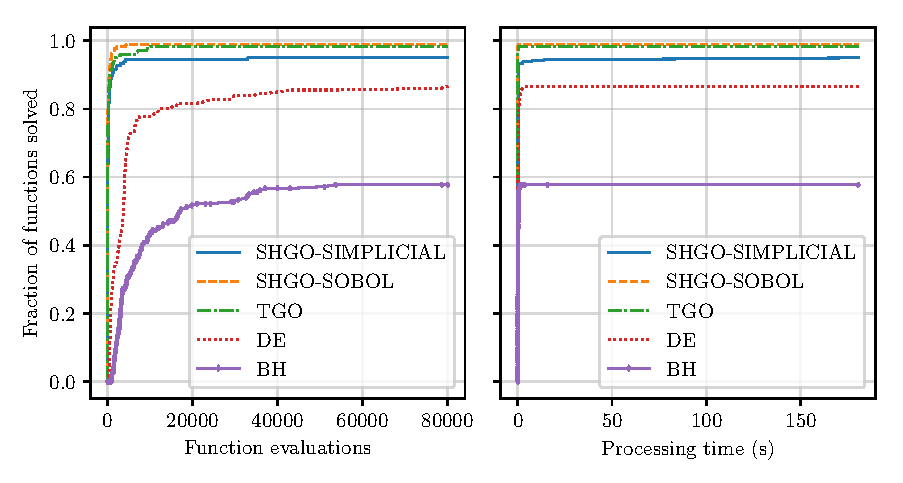
\includegraphics[scale=1.0]{./Fig12.pdf}}
{\caption{Performance profiles for SHGO, TGO, DE and BH on SciPy benchmarking test suite} \label{fig:pprofile}} 
\end{figure}

\begin{figure} %\label{fig:resmin}
\centerline{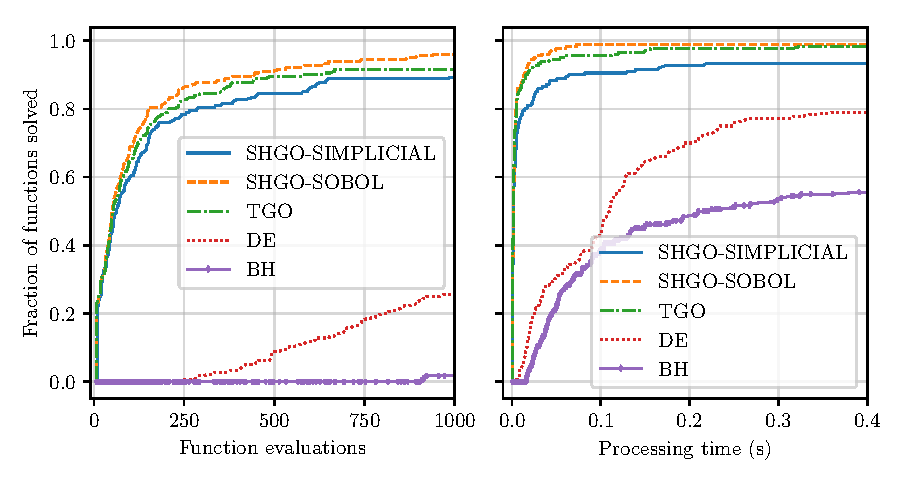
\includegraphics[scale=1.0]{./Fig13.pdf}}
{\caption{Performance profiles zoomed in to the range of $f.e.=[0, 1000]$ function evaluations and $[0, 0.4]$ seconds run time} \label{fig:pprofilezoom}} 
\end{figure}

\section{Invariance and optimum minimiser pool}
The following 4 optimisation test problems were used to demonstrate the applications of \Cref{theorem:invariance_M} and to show the minimiser pool growth compared to TGO over a large number of sampling points. The results plotted in \Cref{fig:resmin} shows that SHGO performed as expected with the minimiser pool staying at the optimum cardinality to map all the local minima once the sampling is adequate as well as the shortcomings of the TGO especially in the higher dimensional test problems where the the minimiser pool tends to grow rapidly with the number sampling points $N$.

The Ursem01 function for two dimensions is defined as follows \citep{Gavana2016}
\begin{equation} \label{eq:Ursem01}
f(\bold{x}) =  \displaystyle - \sin{\left(2 x_1  - 0.5 \pi \right) - 3 \cos{\left(x_2\right)}} - 0.5 x_1 , ~ \bold{x} \in \Omega =  [0, 9] \times [-2, 2] 
\end{equation}

The paraboloid function for six dimensions is defined as follows %\citep{Gavana2016}
\begin{equation} \label{eq:Paraboloid }
f(\bold{x}) =  \displaystyle \sum^6_{i=1} x_i^2, ~ \bold{x} \in \Omega =  [-10, 10]^6 
\end{equation}

The Bird function for two dimensions is defined as follows \citep{Gavana2016}
\begin{align} \label{eq:Bird} \nonumber
f(\bold{x}) =& \left(x_1 - x_2\right)^{2} + e^{\left[1 -
         \sin\left(x_1\right) \right]^{2}} \cos\left(x_2\right) + e^{\left[1 -
          \cos\left(x_2\right)\right]^{2}} \sin\left(x_1\right), \\ 
          &\bold{x} \in \Omega = [-2\pi, 2\pi]^2 
\end{align}


The Schwefel01 function for six dimensions is defined as follows \citep{Gavana2016}
\begin{equation} \label{eq:Schwefel01}
f(\bold{x})= \left(\sum_{i=1}^n x_i^2 \right)^{\sqrt{\pi}} , ~ \bold{x} \in \Omega = [-100, 100]^6
\end{equation}

\begin{figure} %\label{fig:resmin}
\centerline{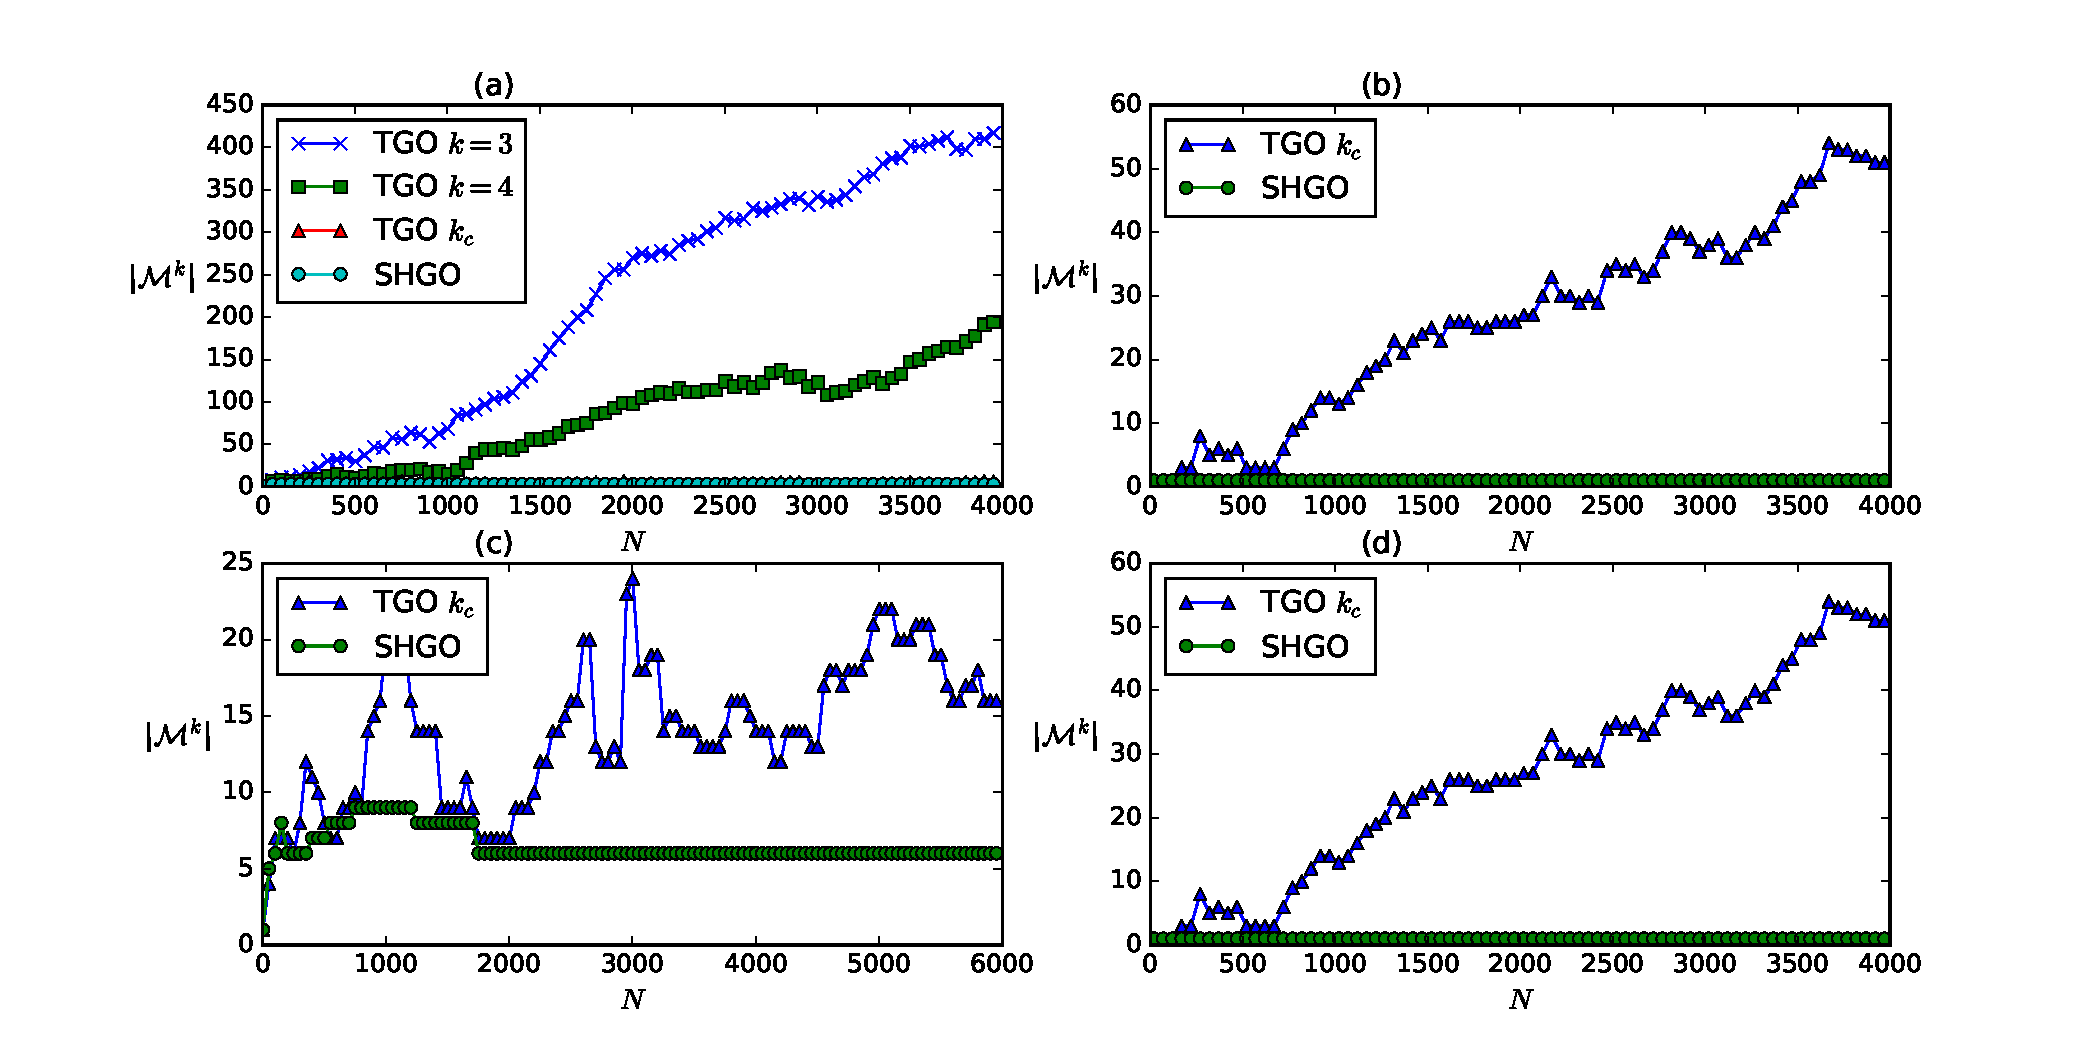
\includegraphics[scale=0.6]{./Fig11.pdf}}
{\caption{(a) The minimiser pool growth of the TGO and SHGO algorithms for the smooth objective function described in Example 3 and restated in Equation~(\ref{eq:Ursem01}) for convenience, the SHGO never increases above the optimum of $|\mathcal{M}| = 3$, for TGO 3 different values of the $k$ parameter are shown. (b) The minimiser pool growth for the six-dimensional paraboloid problem defined by Equation (\ref{eq:Paraboloid }), note that even though the problem has only one minimum, the minimiser pool for TGO set at $k = k_c$ tends to increase for increasing sampling points $N$. In general this problem is exacerbated in higher dimensions while SHGO stays at the optimum $|\mathcal{M}| = 1$. The TGO minimiser pool for $k = 3$ and $k = 4$ are not shown here because the minimiser pool grows too rapidly. (c) The minimiser pool growth for the two dimensional Bird problem defined by Equation~(\ref{eq:Bird}), an important observation here is that $|\mathcal{M}|$ is higher than optimum for SHGO before the sampling is adequate as defined by Equation~(\ref{theorem:invariance_M}) which happens at the after there are $N = 1722$ Sobol sequenced points after which $|\mathcal{M}|$ stays at the optimum value equal to the number of unique local minima with increasing $N$. (d) The minimiser pool growth for the six dimensional Schwefel01 problem defined by Equation (\ref{eq:Schwefel01}), here again $|\mathcal{M}|$ for TGO set at $k_c$ grows rapidly with $N$ while $|\mathcal{M}|$ for SHGO stays constant at the optimum.} \label{fig:resmin}} 

\end{figure}

%In the Table~\ref{tab:results} ndim = $n$ refers the the number of dimensions, nfev refers to the total number of function evaluations used to solved the problem, nlmin refers to the number of local minima found while nulmin refers to the number of local minima that are unique to a set tolerance, success refers to whether or not the algorithm successfully found the correct global minima and finally runtime is the total time the algorithm ran on an optimisation problem measured in seconds.

%\Cref{sec:nres}


%!! TODO: Lennard-Jones crystals \citep{Chill2014} where we have, using function evaluations as a metric, SHGO was 36.5 times faster than BH, 79.6 times faster than DE and 2.6 times faster than our own in-house version of TGO in solving $n = 6$, simulate for the $n=3 \times 60$ using the symmetry constraints.

%!!TODO: Move to an appendix
